\documentclass{article}
\usepackage{framed}
\usepackage{scrextend}
\usepackage{xcolor}
\usepackage[spanish,es-tabla]{babel}
\usepackage[dvips,a3paper,centering,margin=2cm]{geometry}
\usepackage{multicol}
\usepackage{subcaption}
\usepackage[utf8]{inputenc}
\usepackage{color}
\usepackage{float}
\usepackage{cite}
\usepackage{colortbl}
\usepackage{tabulary}
\usepackage{multirow}
\usepackage{amsmath}
\usepackage{graphicx}
\usepackage[breaklinks=true,hidelinks]{hyperref}
\definecolor{shadecolor}{RGB}{25, 133, 161}
\definecolor{rb}{rgb}{0.025,0.5,0.9} 
\definecolor{na}{rgb}{0.8274,0.305,0.196} 
\definecolor{title}{RGB}{0, 23, 31}
\definecolor{ver}{RGB}{255,255,255}
\pagestyle{empty}
\def\to{\rightarrow}
\begin{document}
\vspace*{-2cm}
\changefontsizes{14pt}
\hspace*{-1cm}
\begin{minipage}{0.2\linewidth}
\vspace{0.7cm}
\vspace*{-0.15cm}
\includegraphics[scale=0.12]{images/ifir.eps}
\end{minipage}
\vspace*{-0.4cm}
\begin{minipage}{0.6\linewidth}
\vspace*{0.7cm}
\begin{center}
\changefontsizes{15pt}
\hspace*{-0.1cm}
\textbf{\textcolor{title}{Análisis del PM$_{10}$ medido y el AOD$_{550nm}$ estimado a partir de las mediciones de irradiancia solar VIS-NIR en el Área Metropolitana de Monterrey}}
\end{center}
\vspace{-1cm}
\begin{center}
\changefontsizes{11pt}
Gamaliel López-Padilla$^1$, Adriana Ipiña$^{2}$, Constanza Zuñiga Villareal$^{1}$,Rubén Piacentini$^{2}$\\
1. Facultad de Ciencias Físico-Matemáticas,UANL, México\\
2. Instituto de Física Rosario,CONICET-UNR, Argentina\\
email: giovannilopez9808@gmail.com y ipina@ifir-conicet.gov.ar
\end{center}
\end{minipage}
\begin{minipage}{0.2\linewidth}
\hspace*{0.2cm}

\includegraphics[scale=0.2]{images/fcfm.eps}
\end{minipage}
\vspace{0.2cm}
\changefontsizes{12pt}
\begin{center}
\begin{shaded}
\textbf{\textcolor{ver}{Introducción}}
\end{shaded}
\end{center}
\begin{minipage}{0.47\linewidth}
\begin{figure}[H]
\centering
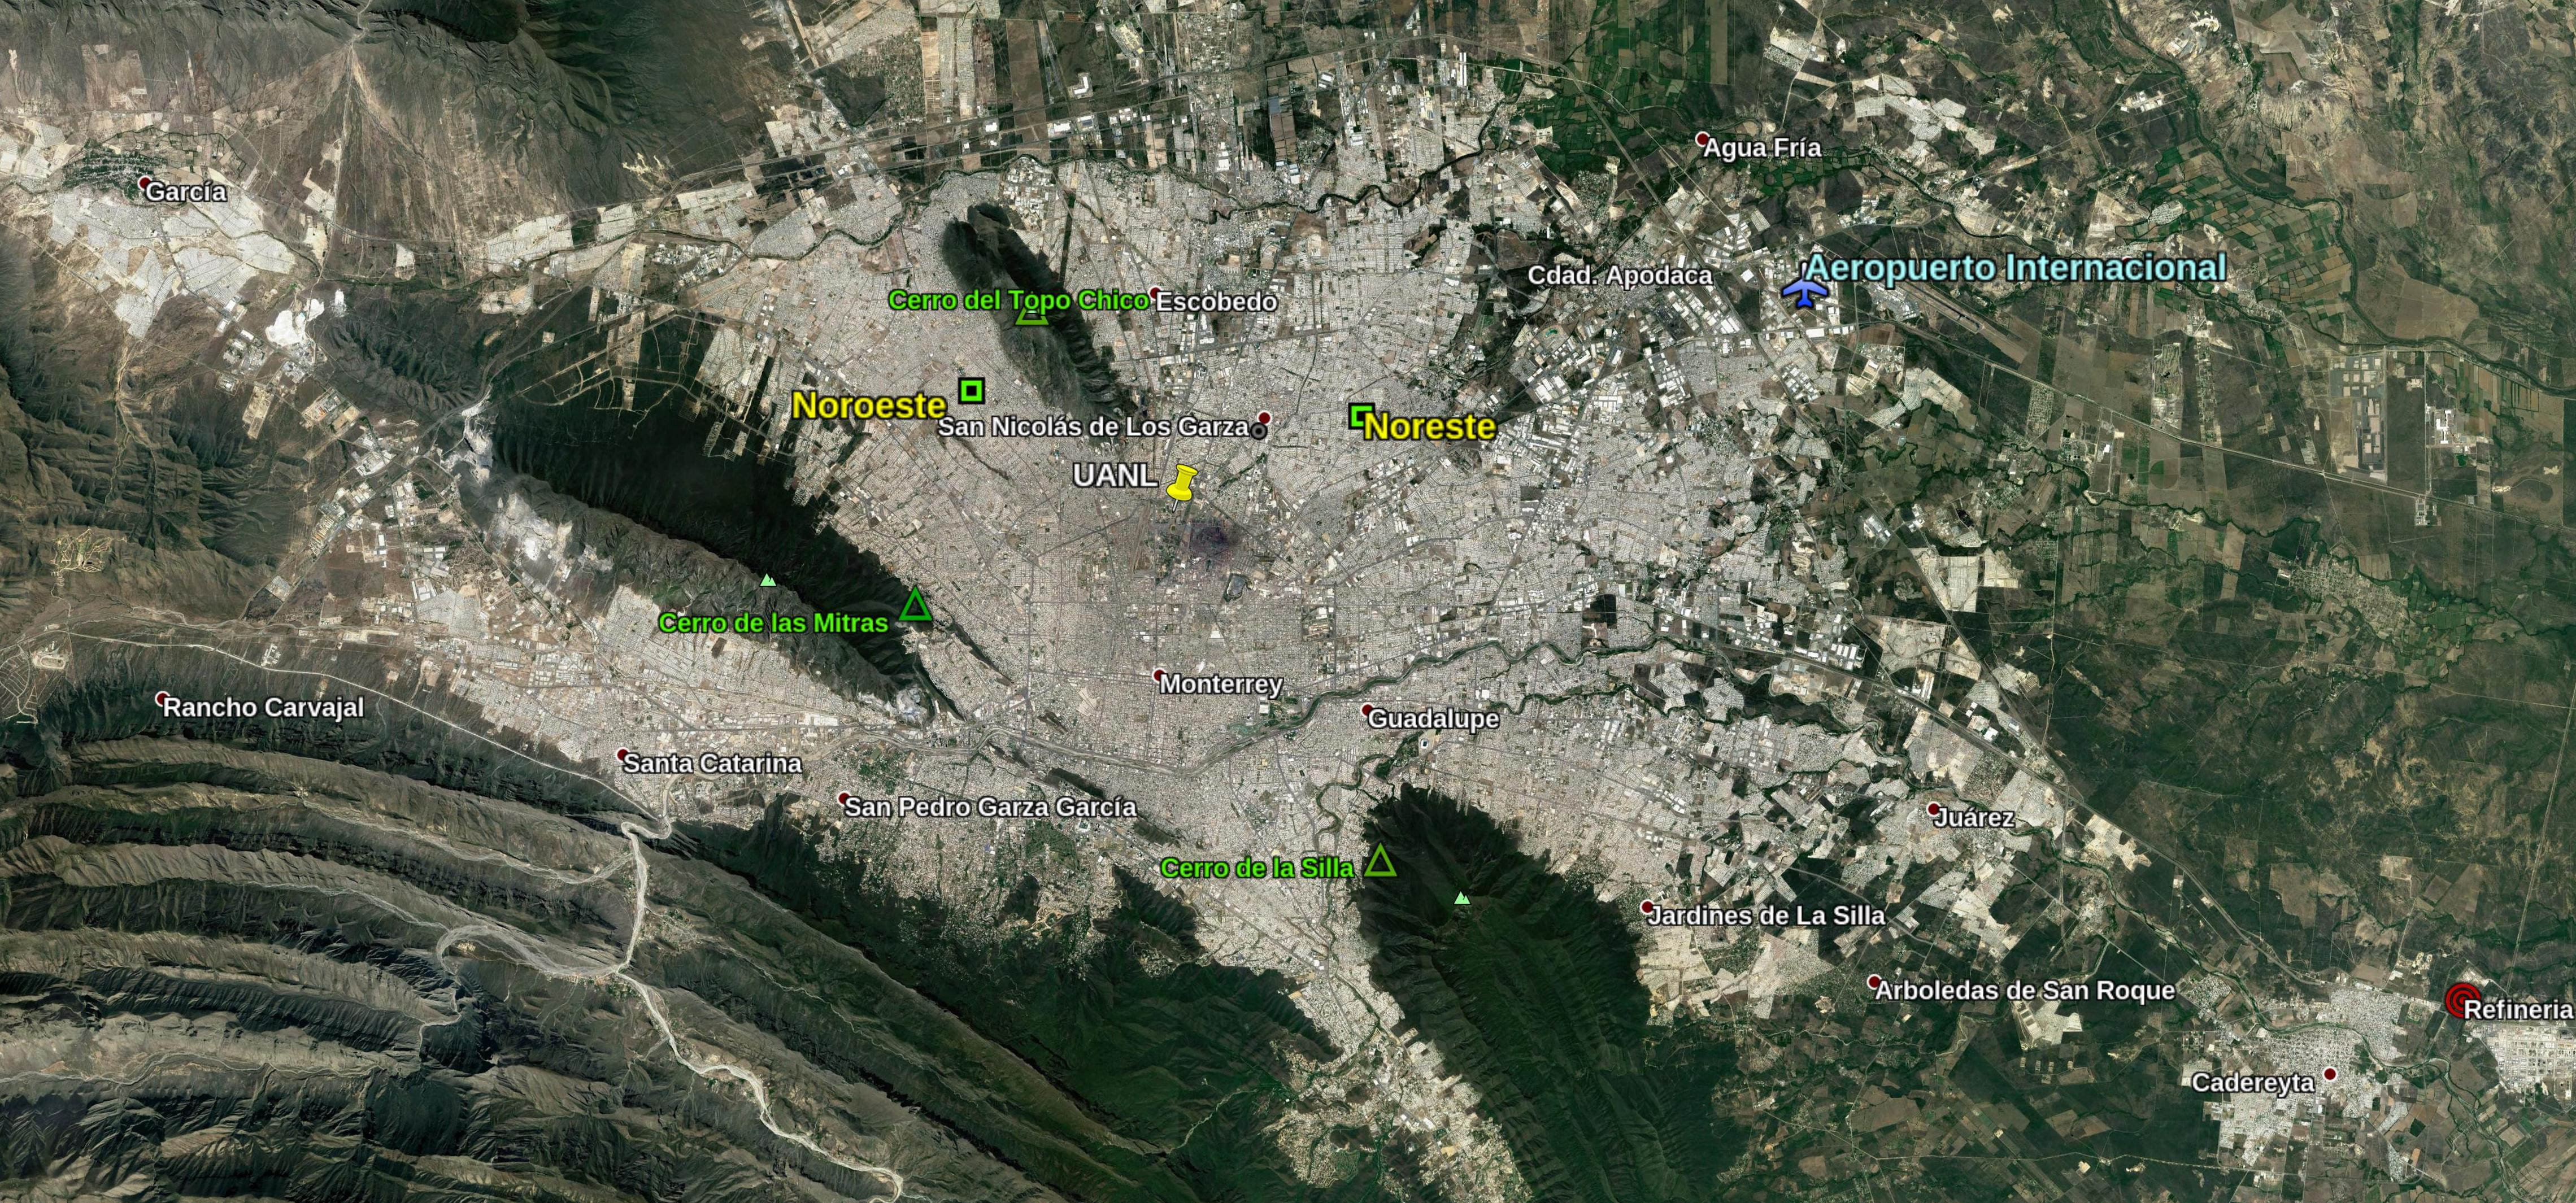
\includegraphics[scale=0.101]{images/satelite.jpg}
\caption{A}
\end{figure}
\end{minipage}
\begin{center}
\begin{shaded}
\textbf{\textcolor{ver}{Metodologia}}
\end{shaded}
\end{center}
\begin{center}
\begin{shaded}
\textbf{\textcolor{ver}{Resultados}}
\end{shaded}
\end{center}
\begin{minipage}{0.60\linewidth}
\begin{center}
\begin{shaded}
\textbf{\textcolor{ver}{Conclusiones}}
\end{shaded}
\end{center}
\end{minipage}
\hspace{1cm}\vspace{0.5cm}
\begin{minipage}{0.35\linewidth}
\begin{center}
\begin{shaded}
\textbf{\textcolor{ver}{Referencias}}
\end{shaded}
\end{center}
\end{minipage}
\end{document}